
The form of sampling chosen was to record all language use by a single subject, across a given period.  As this study is largely exploratory, seeking to drive and refine the methods used, an iterative design was chosen.  This saw a number of preliminary sampling periods, with a review after each to identify the strengths and weaknesses of each.

The subject chosen was myself---this was done for a number of reasons:

Firstly, legal and ethical issues surrounding recording and review of the data were mitigated by having the analysis performed by a member of the original conversations, etc.

Secondly, iterative review of methods involved was possible with internal, `white box' examination of how data were collected, and what edge cases and procedural difficulties arose.

Thirdly, the demographic status and other person-related variables are well known and need no formal elicitation, minimising time spent on construction of questionnaires et al.


\subsection{Data Sources}
Before the first iteration of the sampling/review process, all of the possible language data sources used in everyday life of the subject were informally identified.  It soon became clear that these data sources exhibited properties that would make sampling easier, or less intrusive.  They were classified by the methods required to capture their text:

\begin{itemizeTitle}
    \item[Persistent] Resources that exist in a format that is easily retrieved and immutable.  This covers many physical items such as books, and some broadcast media as well as notes made in a notebook.  Only identifying information must be stored during sampling itself, in some cases merely an ISBN or similar index code.
    \item[Ephemeral] Language data that cannot be accessed after-the-fact in any way, or may differ by time or context.  This most obviously contains speech, but also many websites, things such as billboards that cannot be readily re-accessed, or todo lists that get destroyed.
    \item[Digital Origin] Documents that are read, or written, on electronic devices.  These may fall into either of the above categories, yet they may usually be copied with no overhead so it is often simpler to store them at the time of use.  Many document types are now digital, as well as the obvious sources such as email or online chat.
\end{itemizeTitle}

This classification was useful in order to minimise the intrusiveness of a collection method, whilst maximising the detail recorded for a given source (ideally to the point of storing verbatim text).  In practice, methods were easy to develop for automated recording of digital documents, and many techniques exist for sampling non-digital persistent and ephemeral sources with scientific levels of accuracy already.

Sources initially identified by introspection are listed in black in Figure~\ref{fig:personal:datasources}.

\begin{figure}[p]
\centering
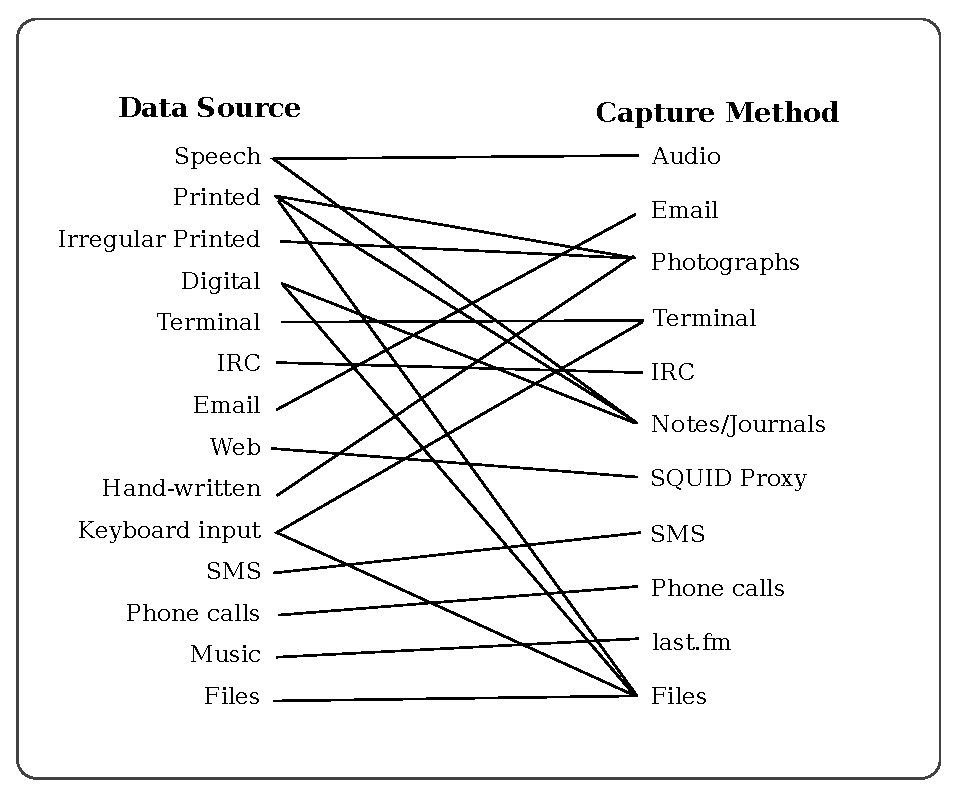
\includegraphics[width=0.7\textwidth]{personal/sources}
\caption{Data sources and their appropriate capture methods (those in blue were added during preliminaries)}
\label{fig:personal:datasources}
\end{figure}



The inadequacies of introspective methods to identify these soon became apparent during preliminary tests, as the process of recording increased awareness of language use, raising a series of edge cases.  These were collected and resulted in a final selection of sources displayed below.  As well as expending the set of sources to be gathered, methods of collection were chosen with flexibility in mind in order to cope with unenvisaged sources of data\footnote{This flexibility has the unwelcome effect of slowing down analysis later on, and may be undesirable in some cases}.


% \begin{itemize}
%     \item Speech
%     \item Printed documents (i.e.\ letters, brochures)
%     \item Digital documents (same, but unprinted)
%     \item Terminal logs
%     \item IRC logs
%     \item Email
%     \item Websites
%     \item Unusually formatted printed material (posters, labels, advertising on vehicles, billboards, etc.)
%     %---
%     \item Written (but non-OCRable) material
%     \item Key strokes
%     \item SMS records
%     \item Phone conversations (separated from speech as they yield differing metadata)
%     \item Music tracks
%     \item Files accessed
% \end{itemize}

The list shown in Figure~\ref{fig:personal:datasources} is necessarily furnished according to the life of the subject in question---from this study I am unable to assert that it is generalisable to others, though the process of doing so would involve relatively little intrusive sampling\td{link to further work}.

Each of these sources is ``covered'' by one or more sampling tools.  These tools progressed most during the iterative process, and each was subject to a number of procedural subtleties that were refined throughout the study.










\subsection{Recording Methods}
Method used to record data were chosen for a variety of reasons.  They must, in sum, cover the sources mentioned above, be unobtrusive both for the experimenter and those around him, and be sufficiently flexible to cover unforseen contexts and data sources.

These methods can be separated further into two groups: many methods are capable of recording multiple sources, and serve to form a narrative that describes the metadata of a linguistic event, pointing at another source for the data itself.  These methods were chosen to allow for post-hoc sensemaking and narrative creation, something that was added to the experimental procedure after the first iteration indicated how difficult to operationalise much of the data would be.

The second set of methods are focused on a single data source, typically requiring little to no manual intervention to record data.  Their records are either indexed by time, or by the more flexible methods mentioned above.


\subsubsection{Indexing and Overview}
\paragraph{Journals and Note-taking}

\begin{figure}[p]
    \centering
    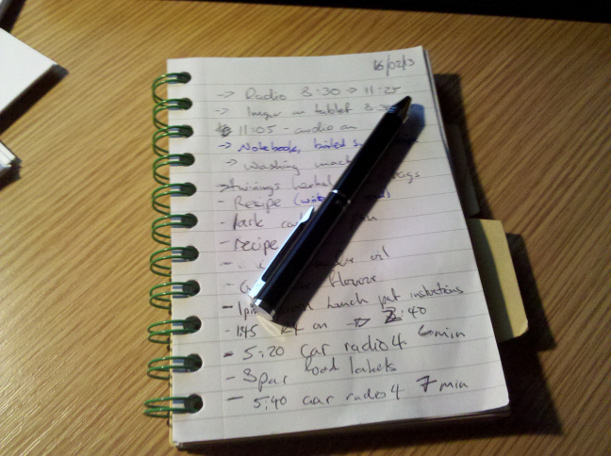
\includegraphics[width=0.8\textwidth]{personal/notebook}
    \caption{The `on-line' notebook}
    \label{fig:personal:online_notebook}
\end{figure}

Two journals were maintained throughout the sample.  The former of these was an A6 notebook maintained `on-line'\td{rename to hot/warm/cold, front/mid/backline or something similar} as events occurred (pictured in figure~\ref{fig:personal:online_notebook}).  This was used to store durations of conversations, titles of persistent sources, etc.

The second was an off-line journal, maintained at the end of each day in a narrative style.  This blog-like record was intended to reflect in depth on the proportions of text used in each source, and how attentively each linguistic event was engaged in.  The writing of the journal itself was not logged by any other methods.  It was also possible to attach daily records to this journal, and the process of writing it inserted an opportunity to reflect on the mnemonic codes used during the day.  This process is described in context in section~\ref{sec:personal:recording}.

The on-line notebook proved to be the primary indexing method for all other sources of data, and its maintenance was the primary overhead of the study.  As illustrated in Figure~\ref{fig:personal:notebookformat}, each entry in the notebook was eventually reduced to a compressed form that roughly followed one-line-per-event, storing the time each event occurred, any identifying information deemed necessary for later memory of it, and a duration or other index of word counts.

\begin{figure}[p]
    \centering
    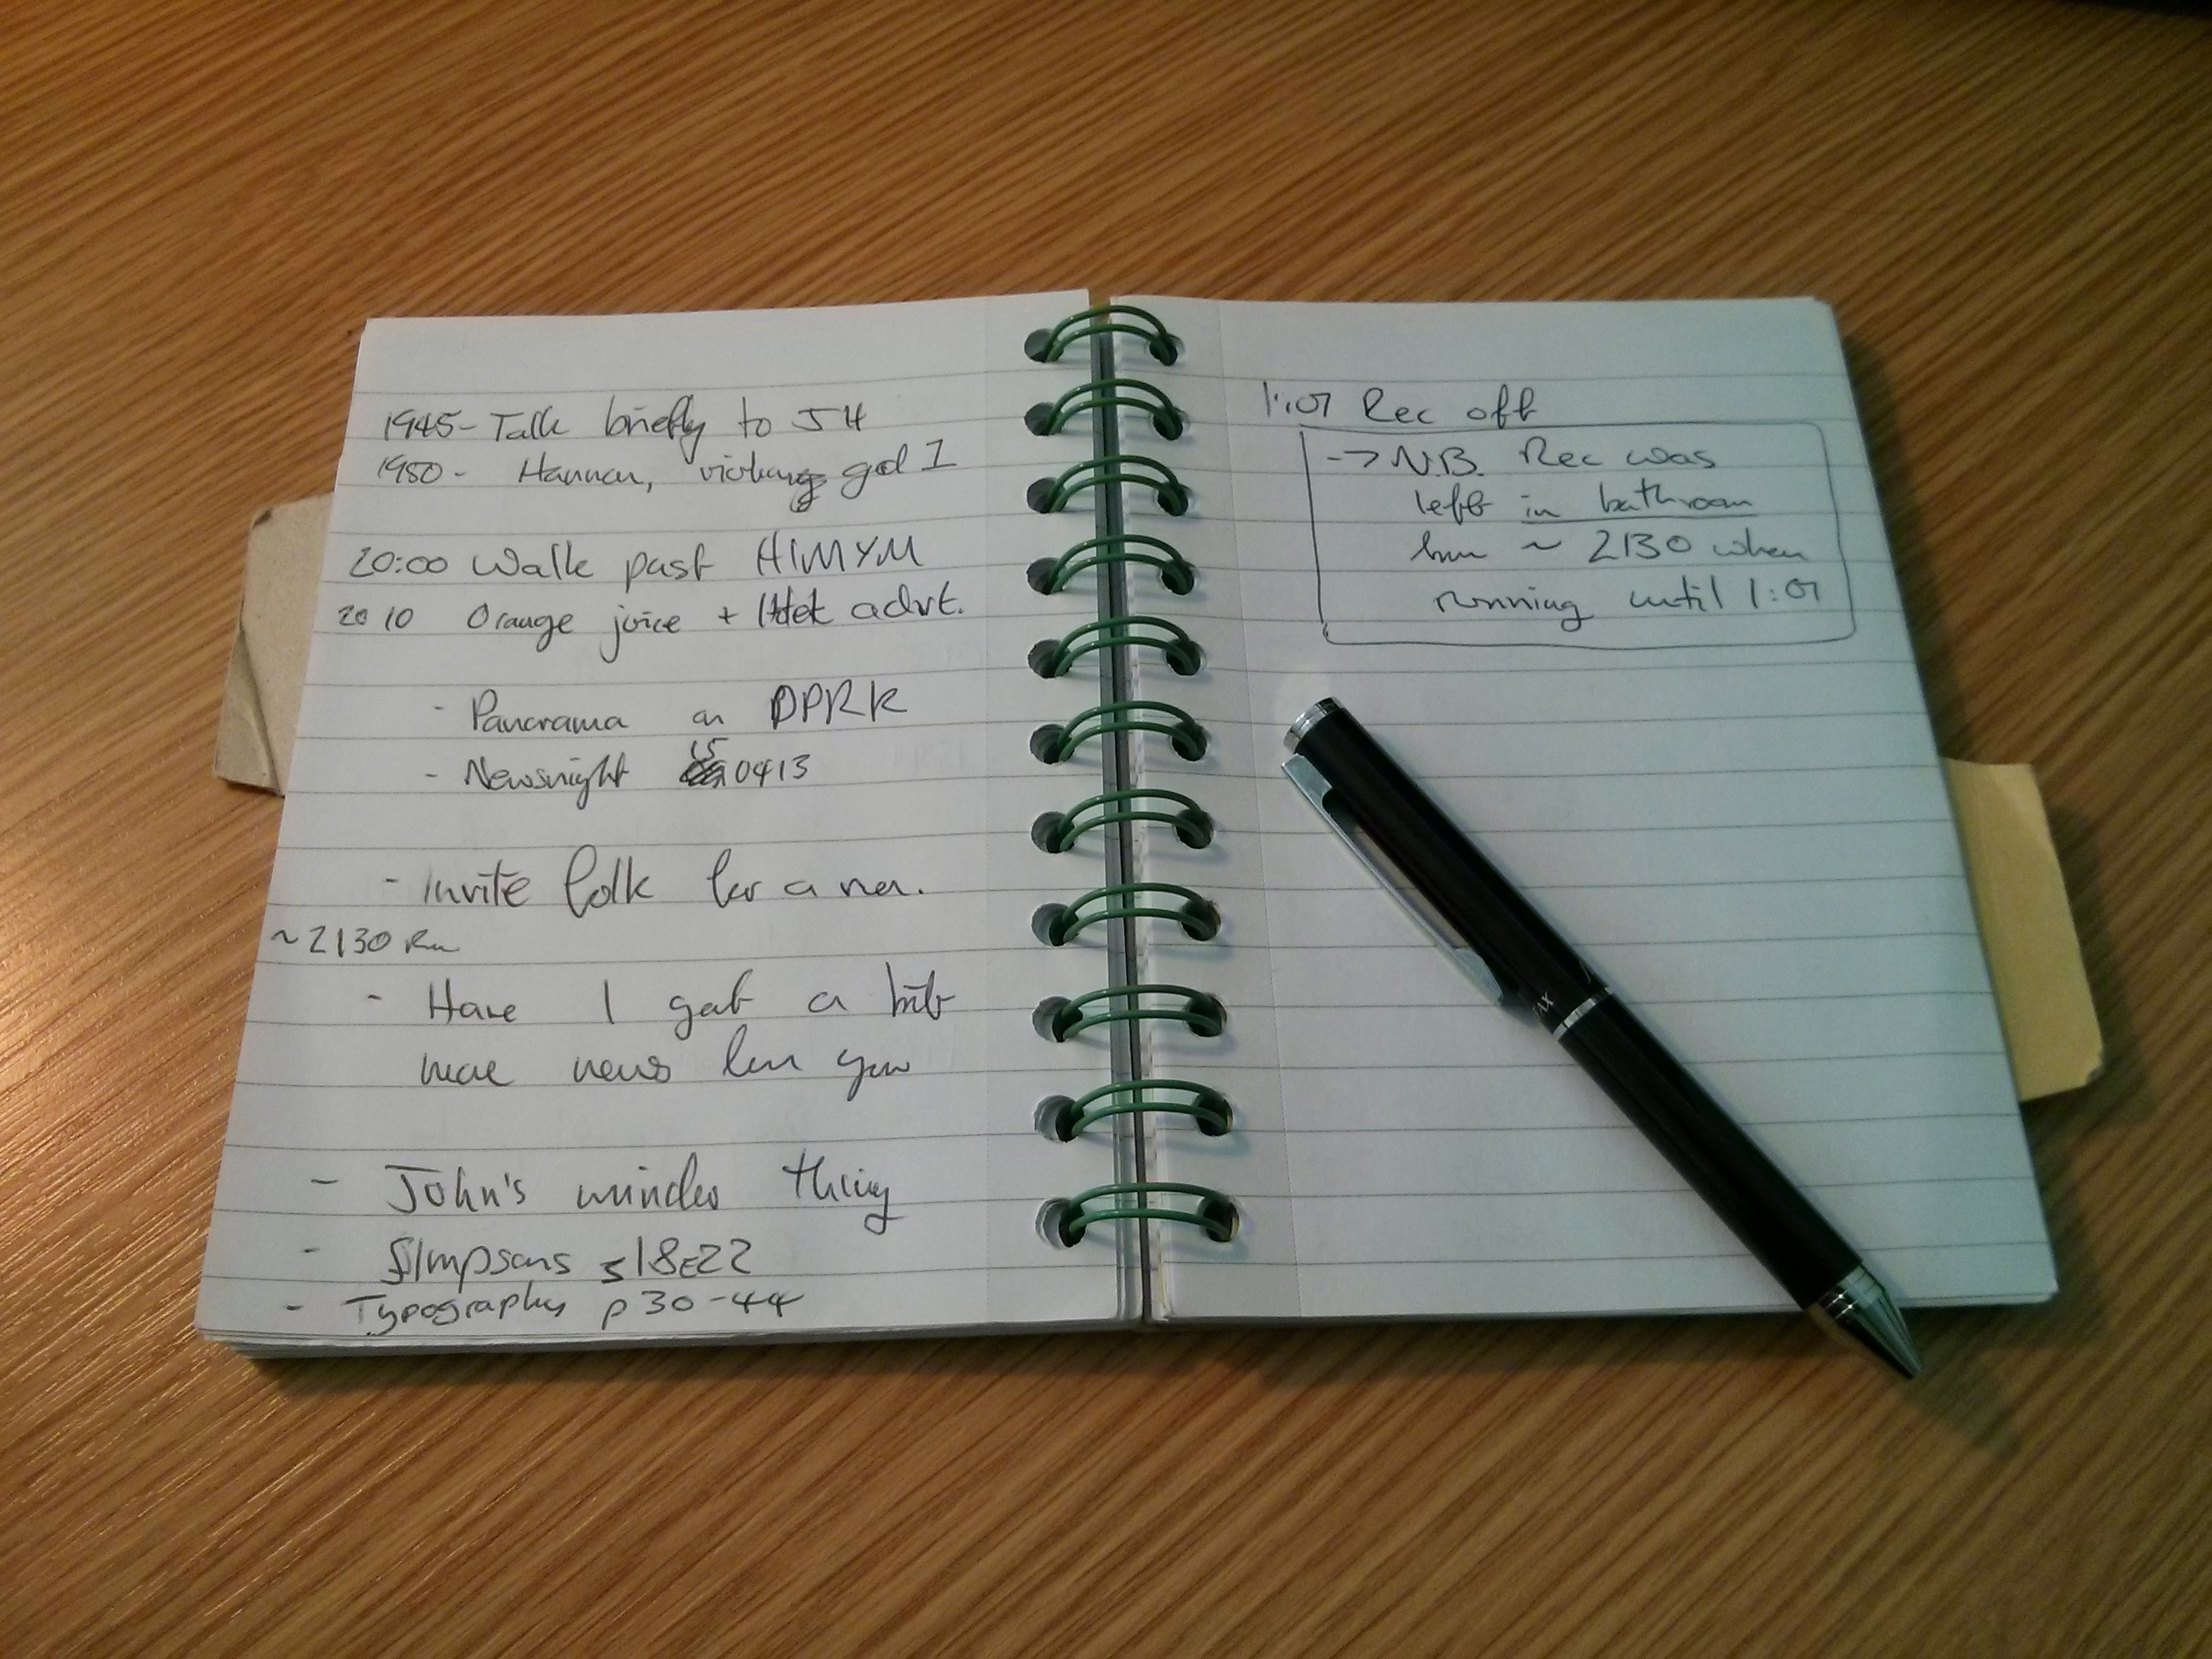
\includegraphics[width=0.8\textwidth]{personal/notebookpage}
    \caption{A page from the on-line notebook, detailing the format used}
    \label{fig:personal:notebookformat}
\end{figure}


Problems of simultaneous events and split attention were solved in the notes by having a start/stop event for ongoing events, and by using the off-line journal to reflect upon each event.

\paragraph{Audio Recording}
Following work on machine listening, the original intent of audio recording was to capture the occurrence and duration of conversations, as well as any smaller interactions that would otherwise be difficult to capture (such as greetings, thanks when opening doors, etc.)


\begin{figure}[p]
    \centering
    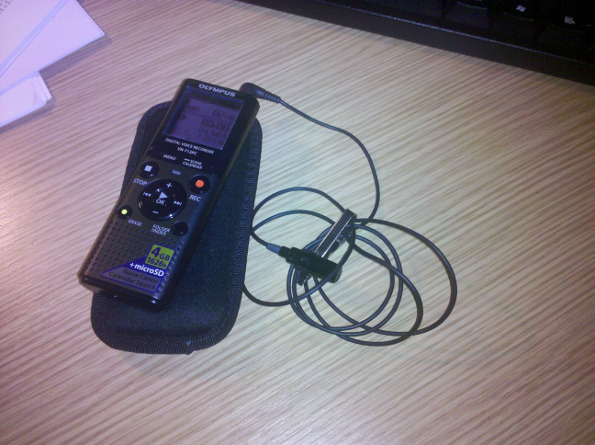
\includegraphics[width=0.8\textwidth]{personal/dictaphone}
    \caption{The audio recorder used}
    \label{fig:personal:audiorecorder}
\end{figure}



Capturing was performed with an Olympus VN713PC dictaphone, recording to a suitably sized external card that yielded many days' continuous recording.  Provision was made to download recordings each night and store them with the off-line journal, however, in practice they remained on the recorder until the end of the study.


\begin{figure}[p]
    \centering
    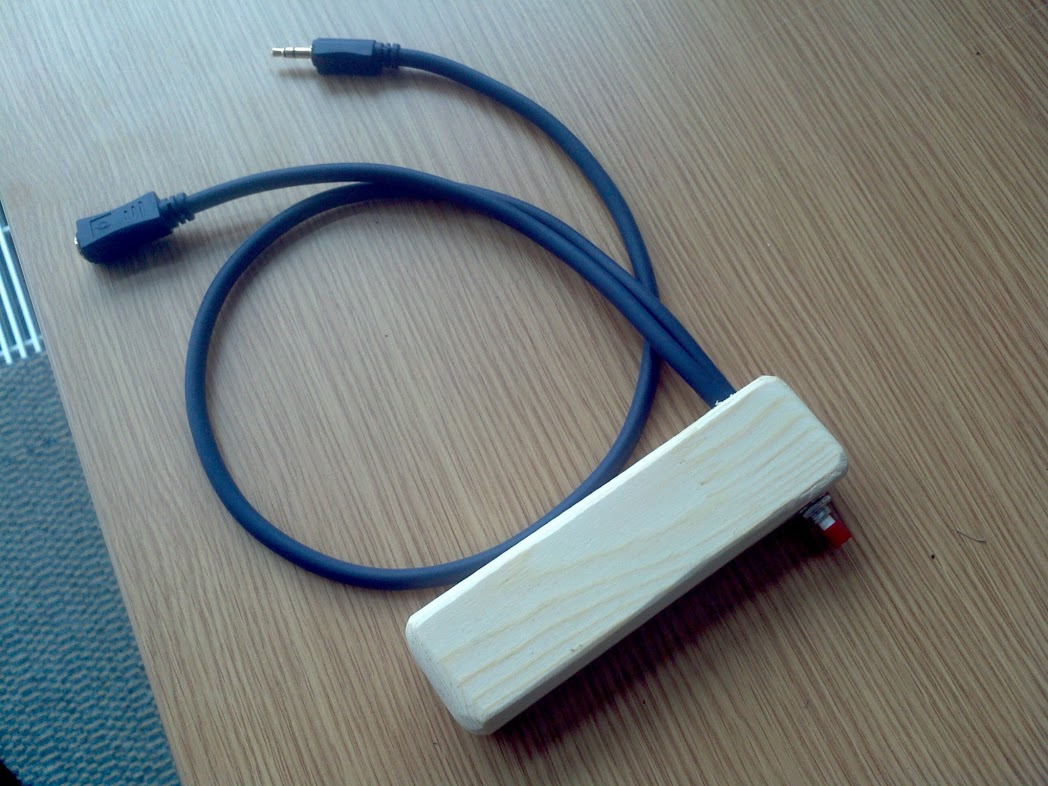
\includegraphics[width=0.8\textwidth]{personal/clicker}
    \caption{The second audio index marker}
    \label{fig:personal:clicker}
\end{figure}


Aligning the recorder's output to the events mentioned in the notebook was a tricky process---Though the recorder itself supports index marks, there is a limit of 99, which was deemed riskily low.  Two devices were built to insert absolute silence onto the recording (something that is rare in real life and easy to programmatically detect), the later of which is pictured in figure~\ref{fig:personal:clicker}.  These clickers were to be pressed at the beginning of each conversation, so that voice activity detection could be performed to estimate the word count of each conversation (or, in an ideal world, extract verbatim text).

In practice, the process of tapping the button proved intrusive and, from the perspective of one talking to the subject, suspicious.

The mechanism used for the final iteration of the study was far simpler---the recorder's start time was written in the on-line notebook, and entries therein were keyed by computing the offset between the two times.  Though this incurs a minor overhead in coding the data, it also allows for spontaneous conversations without much overhead, something that is particularly important to the study of text type proportions.



\paragraph{Photographs}
The primary method of capturing ephemeral, irregularly formatted, non-digital texts was photography using a cameraphone.  This method was chosen largely because the ubiquity of smartphones in British society has led to a situation where photographing fairly mundane items is widely unquestioned.

The smartphone used, a Motorola Milestone, also stores time and location data in its photographs using EXIF tags (as well as storing photographs sorted by day).  This metadata meant that there was often no need to file an entry in the on-line notebook, and the cameraphone could simply be used in a very unobtrusive ad-hoc manner.

In earlier iterations of the study, it became apparent that the loud shutter noise made by the Android operating system when taking photographs was problematic.  Though photography of signs, packets and such remained unchallenged, the attention of people nearby was drawn to the weirdo with the cameraphone all too readily.  This was solved partially by (with great difficulty) disabling the noise, though it was still apparent from posture when a photograph was being taken.

There are notably a number of products available that continually take photographs for the purposes of life logging.  These were considered for the study, but their aims are generally to capture each event, rather than specific aspects of selected scenarios.  The ability to consciously specify that the subject was more attentive in some situations (and take pictures accordingly) was judged to outweigh the value of having a continuous record (something much more capably performed by the journals).




\subsubsection{Targeted Methods}
\paragraph{Phone Calls \& SMS Messages}
Both of these are automatically logged by the Android operating system used by the subject, and each was also indexed in the on-line notebook.  The data was extracted using a free application that exported to XML.


\paragraph{IRC}
IRC was logged by construction of a bot.  This bot accompanies the subject into chatrooms and logs all messages observed, applying a rough human interest model to ignore data seen when the user is set to away.


\paragraph{Web}
The SQUID webproxy was configured to log all traffic, and a number of logins were provided---one for each of the subject's internet-enabled devices.

The logs from SQUID store all requests, including advertising/tracking calls, downloading of things never read by the user (i.e. CSS and Javascript) and AJAX calls to partially reload pages.  As such, a large amount of processing was necessary to extract URLs from these logs, and to parse the resultant data into a usable format.

\paragraph{Keylogging/Terminal recording}
Terminals and keyboard input were logged using a custom application that wrapped a terminal, recording the time each character was sent or received to the shell.

Each terminal created started recording to a new log file, storing the time at which it was started and a series of offsets from this time.

\paragraph{Last.fm}
In earlier iterations it was apparent that lyrics in music were being missed as a source of text---all devices capable of playing music were configured to `scrobble' to the last.fm music service during the sampling period.

Though last.fm do not make their data freely available for access, third party tools exist to scrape their website and download detailed logs of tracks listened to.

\paragraph{Files}
Files were identified in a number of ways.

Some, particularly those on which the subject worked and contributed data, were written down in the journals.  This is a precise method of separating what has been read, but might require a large overhead.

Since the subject works entirely on projects and files that reside in a RCS repository, the logs from each commit were used to generate a diff, and this was accessed after the sampling period to identify contributions made.

Another policy that may be used is identification of files by unix mtime (modification) or ctime (creation), however, this is fraught with inaccuracy, as files are liable to be modified on disk many times whilst being edited, and sampling the differences is likely to happen at haphazard times.  Further, this technique would capture many log files and others that have been edited by processes where the subject was not involved linguistically.  By contrast, commits to an RCS are scheduled around logical additions, and are manually pushed so that only deliberately edited files are stored.

Files uploaded whilst on other systems may be uploaded directly to the off-line journal (which, ironically, is online), or stored on a flash drive that was carried specifically for the purpose.  In practice this did not occur during the recording period, though experience suggests these contingencies would be necessary if a longer sample were taken.

\paragraph{Email}
Emails are, again, stored automatically with sufficient metadata as to make them self-documenting.  However, rather than presume all were read in a given day, each was tagged after being read with a label corresponding to the day.

At the end of the sampling period, these tags were collected and downloaded in mbox format, whence they were processed by the operationalisation script.









\subsection{Recording Procedure}
\label{sec:personal:recording}
The study is based around a period of continuous sampling using the methods discussed above.  For two weeks (in some cases longer), data was captured for each source.  This process was structured around a daily routine:

Upon waking, and before any language was used, the recorder was turned on and a note of the time at which this occurred was made in the on-line notebook.  Recording was then continued until the end of the day without interruption.

The on-line notebook, smartphone, and flash drive, were carried at all times.  Since each of these could be backed up (the smartphone even did this backup automatically), the most data at risk was a single day.

Notebook entries were made as soon as was possible without interrupting the linguistic event being recorded.

At the end of the day (immediately prior to sleep), a journal entry was written in the off-line journal, and SQUID logs were uploaded for the day.  This journal entry forms a narrative, estimating the time taken and attention paid to items in the on-line journal for that day, as well as detailing anything that may be written in shorthand-mnemonic form.










\subsection{Operationalisation, Processing and Analysis}
Normalising and operationalising such heterogenous data without significant overhead proved to be a significant problem that was only partially solved, and the data set presented here required significant manual intervention that was possible in part due to the fact that the analyst was the subject.

This advantage, clearly, cannot be relied upon in other studies, and this part of the method demands most further study in order to define typical parameters for many processes that are dependent on human properties.

Two main processes were followed in data processing.  The former of these was aggregation and normalisation---each data source was collected and transformed into a one-event-per-line CSV containing a standard set of fields (the selection of fields used was modelled on Lee's BNC index\td{CITE} in order to facilitate comparison).

After this normalisation process was complete, data were manually annotated to complete any fields that were not stored in the original metadata.  This was largely an objective, uncreative task that simply demanded human reasoning capacity, but it is inevitable that some bias will creep in at this stage.

The second stage of processing involved coding text types and roles.  This task is altogether more flexible and subject to design errors and bias than many of the normalisation stages, and was thus attempted in a manner that was designed beforehand.  Since the aim of this study is, in part, to identify text types not seen in other corpora, following an existing taxonomy would necessarily limit the coding of any newly discovered.  True free coding, however, is likely to draw distinctions between text types that are not made in existing taxonomies, rendering them incomparable.

The process followed was a hybrid approach---data were freely coded by inspection of the texts, but this was done with deliberate prior knowledge of Lee's classification scheme.  The intent was to categorise texts according to Lee's scheme only in so far as they were deemed suitable by the analyst (who is also, lest we forget, the subject).

Though this approach was suitable for the aims of this particular study, it is difficult to advocate for any others using the sampling techniques described, and its use here should not be taken as such.

%---
\subsubsection{Human Interest Models}
Beyond coding, by far the largest single influence on the data recorded was the human interest model applied.  This was created in order to take into account two factors that had become particularly apparent (and notably do not apply in the same manner to conventional corpus designs, where many eyes may cover a whole document in sum):

\begin{itemize}
    \item Often, only small (usually predictable) portions of a text are used.  For example, I have started to read more books than I have finished reading.  Generalised, this means that even Brown-designed corpora should favour the start of their texts slightly when selecting excerpts.  Some media were more surceptible to this than others, and the automated normalisation tools were built with facilities to take this into account.
    \item Texts, especially broadcast media and speech, were often used whilst also accomplishing a non-textual task (or sometimes both at once, such as talking with the radio on in the background).
\end{itemize}

Both of these were noted in journals, and added to the processing toolchain---each data source's normalisation script contained a model to extract the portions of text that were read, and each row of the normalised data format contained an ``attention index'', ranging from 0--1, that served as a coefficient of the word count.

Though crude, this measure was able to produce approximations for word counts that were inline with the expectations of the subject.  (It is recognised that this may not hold much scientific value to others wishing to replicate the study, and in general it is necessary to investigate the inter-person variability of these properties in order to create more generalised processing tools.)


% TODO: perhaps a run-down of each annotation program?
\paragraph{Web logs}
The human interest model for web logging was built by inspection of the web logs and cross-referencing with information about the hosts identified.  The normalisation script is concerned primarily with removing material that was downloaded without ever having been viewed, for example, non-text MIME types and advertising, and contains a multi-stage strategy for excluding content:

\begin{enumerate}
    \item Filter only successful requests
    \item Filter only those requests that are of textual mime types (\texttt{text/*})
    \item Apply a blacklist of advertising websites and file extensions (manually constructed)
    \item Discard links where the page was reloaded and the URL is the same as the previous entry in the list (this pattern is often caused by initially connecting to the proxy, for example)
    \item Non-visible text items were discarded (non-body elements if the file is HTML), and markup was removed
\end{enumerate}

Beyond this initial normalisation, a speadsheet's \texttt{LOOKUP} function was used to manually assign attention coefficients to the domains, based upon entries in the journals and interesting portions of web pages that follow regular structures.

Days were classified as changing at 4am, since there were no points in the data set where the subject was still using the web at this time.



\paragraph{IRC Logs}
IRC logs were already stored using a limited attention model, which was based on the principle that, in IRC, conversations are started, live for a short time, then die off as people in the channel return to work.  The bot performing logging would start logging (and continue to log) for as long as the subject was talking, stopping 10 minutes after the final utterance.

In order to capture a human notion of day, that is, one demarked by sleep rather than midnight, the start time of each conversation was used to determine the day its data fell into.



\paragraph{Terminal [Console] logs}
Terminal data was logged with timestamps on each individual character, and the model was thus responsible for inferring when a command had output, and suggesting which portions of text were still on screen.

This was done with a `timeout' and a `scrollback'---the former describing a delay that had to be present for the text to have been read (rather than simply scrolling offscreen), and the latter describing the average size of a terminal (and thus the number of rows of text that remain displayed).

These parameters were tuned to match the specific data sampled over the period---for example, the time recorded included terminal use displaying logs from software that was being developed, and these would produce thousands of lines of output before a pause.




\subsection{Coding and Genres}
Since the case study is in part aiming to identify genre distinctions not found in other general-purpose corpora it is not possible to select, a priori, an authoritative taxonomy of genres.  This problem is further complicated by the mix of spoken and written data in the corpus, something that would usually be more formally separated.

% \til{Also note how I'm coding things from both spoken and written, and such, thus one taxonomy would be unable to cover it anyway?}

Genre distinctions were made using a process that loosely follows the principles of the coding stages of grounded theory \td{cite}.  
This involves a focus on free coding, and a consideration of all available context and information---something aided both by the `memoing' innate in the design of the journals, and the fact that the analyst is also the subject.  Free coding was performed with prior knowledge of Lee's genre categories.


This process was done in order to deliberately apply distinctions made by Lee where these seem appropriate, but to retain the flexibility to deviate where portions of the corpus did not fit comfortably within the existing categories.  This soft alignment was chosen in order to ease comparison against existing corpora, especially the BNC.  No effort was made to adhere to Lee's specification directly, so as to prevent forming a disconnect between the Lee-inspired categories and those that were sufficently different to form their own.
% as this would lead to over-specification where the case study's corpus proves more diverse in form than the equivalent BNC category.

It's particularly noteworthy here that the analyst selecting codes for genres is the same person as the subject gathering the data.  This, along with the mnemonic form of the notebooks and data captured, provides extra (informal) insight afforded by context.


Because of the large volume of data, and the manner in which it was extracted from its original sources, coding was performed using a semi-automated process on a source-by-source basis.  This was chosen in part because the source itself refers to how the language was used by the subject, rather than simply what form it was available to the corpus builder, and is thus a contextual factor affecting genre distinctions.

For data that were processed and annotated largely automatically, codes were assigned after a systematic review of the data itself, using a spreadsheet to reduce the number of lines according to variables that were assumed to define a given genre (for example, web data was split by domain, and music was assigned by artist).  These distinctions were then written into the extraction tools as heuristics, or applied directly before being merged with the main corpus.

For data such as images and notebook entries manual coding was required.  This was completed using similar tools, except that it was seldom possible to reduce the data set before coding, and thus was not possible to apply heuristics to impute data.  Data recorded in these formats were often more varied with many unique or esoteric entires (such as the single tax disc).

In order to better align the informal genre distinctions with Lee's format, the final document genre distinctions were formed by prefixing the data source, i.e. transforming ``rock'' into ``music/rock''.  These resultant genres are used herein for describing the corpus, as as the basis for any direct comparison with Lee's BNC index.

\til{It might still be necessary to review the codes, or align them to Lee's for comparison in the results lower down}


% ---

This process of augmenting manual entries method would, if extended to use external data sources (such as the CDDB music information service), be capable of automatically assigning genres for a number of data sources, greatly easing the manual intervention required.  It is also likely that improvements in computer vision, or applications of existing databases (such as Wikipedia, or the web itself) could be used to extend these methods further to cover images and other data that were manually processed here.
